\documentclass[11pt]{article}
 
\usepackage[T1]{fontenc}
\usepackage[polish]{babel}
\usepackage[utf8]{inputenc}
\usepackage{graphicx} 
\usepackage{lmodern}
\selectlanguage{polish}
\title{Optymalizacja działania algorytmów sortowania - Quick Sort}
\author{Mateusz Bencer, nr: 209360}
\begin{document}
\maketitle
Sprawozdanie zawiera wnioski wyciągnięte z optymalizacji algorytmów sortowania - Quick Sort. Celem pomiarów było sprawdzenie wpływu doboru elementu osiowego (ang. pivot) 
na czas sortowanie określonej liczby elementów w kontenerze. Na potrzeby tego zadania użyłem implementacji listy z programu Łukasza Saka. Doświadczenie z pracy nad cudzym kodem okazało się bardzo pouczające...
\newline
W celu możliwości implementacji algorytmu sortowania konieczne były drobne zmiany w kodzie, tj.:

\begin{itemize}
  \item Musialem dodać metody set oraz get do klasy lista, ponieważ niemożliwym było zaimplementowanie 
  algorytmu, gdzie przy pobieraniu elementu został on ściągany, a podczas dodawania inne zostały przesuwane. Metodom pośredniom (sprawdzoną przeze mnie) było pobieranie wszystkich elementów do zwykłej tablicy za pomocą metody pop, posortowanie tej tablicy, i późniesze powrotne dodanie tych 
  elementów za pomocą metodu push do listy. Jednak jak było to do przewidzenia, miało to bardzo negatywny wpływ na złożoność oraz osiągane rezultaty czasowe. O wiele prostsza byłaby implementacja tego algorytmu na liście powiązanej (linked list), gdzie każdy element zwiera wskaźnik do poprzedniego i następnego elementu, ale na moment kiedy pobrałem kod z gita, była tam tylko implementacja tablicowa.
  \item Musiałem dokonać gruntownych zmian w klasie Benchmark, która była stricte dopoasowana do poprzednionego zadania (mało uniwersalna).
  \item Dodałem zaimplementowaną przez siebie wcześniej klasę Timer do pomiarów czasowych.
\end{itemize}
Zostało przeze mnie przetestowanych 5 sposobów doboru elementu osiowego. Pomiary zostały przeprowadzone dla 9 kolejno rosnących rozmiarach listy. Wszystkie elementy umieszczone w liście są pseudolosowe.
\begin{itemize}

\item 1. Pierwszy skrajny element. \newline
Z rozważań teoretycznych wynikało, że jest to najprostsza, ale zarazem najbardziej naiwna metoda doboru elementu osiowego. W przypadku tablicy wstępnie posortowanej taki wybór może skutkować złożonościa nawet \begin{math}0(n^{2})\end{math}. Moje pomiary (na liście z elementami losowymi) potwierdziły to.
\begin{figure}[ht]
\centering
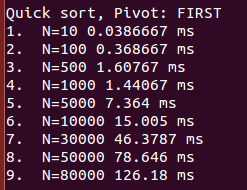
\includegraphics[width=0.35\textwidth]{first.png}
\caption{Wyniki działania programu, gdy piwot jest pierwszym, skrajnym elementem}
\label{fig1}
\end{figure}

\item 2. Ostatni skrajny element. \newline
Wybór ostatniego elementu jest analogiczny do wyboru pierwszego skaranego elementu. W takim wypadku złożość rónież może wynieść \begin{math}0(n^{2})\end{math}. Moje pomiary również dają podobne rezultaty jak do tych z podpunktu 1.
\begin{figure}[ht]
\centering
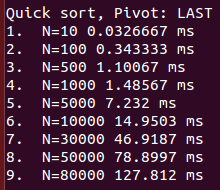
\includegraphics[width=0.35\textwidth]{last.png}
\caption{Wyniki działania programu, gdy piwot jest ostatnim, skrajnym elementem}
\label{fig1}
\end{figure}

\item 3. Element losowy. \newline
Wybór elementu losowego ma na celu uśrednienie możliwości wystąpienia sytuacji najbardziej optymistyczne, jak i najbardziej pesymistycznej. Jest to metoda bardzo zapobiegawcza. Jest złożoność to około T(n) = 2nln(n) (przy rozkładzie równomiernym). Jednak według moich pomiarów jest to metoda gorsza od dwóch poprzednich. Podejrzewam, że jest to związane z dodatkowym nakładem czasowym potrzebnym na wylosowanie elementu.
\begin{figure}[ht]
\centering
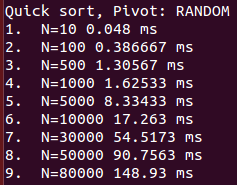
\includegraphics[width=0.35\textwidth]{random.png}
\caption{Wyniki działania programu, gdy piwot jest elementem losowym}
\label{fig1}
\end{figure}

\item 4. Element środkowy. \newline
Taki wybór jest chyba najbardziej popularny, przynajmniej wśród implementacji quick sorta znalezionych przeze mnie w internecie. Zapobiega on występowaniu (w prawie wszystkich przypadkach) sytuacji najbardziej pesymistycznej, a wyliczenie elementu środkowego wymaga małych nakładów obliczeniowych. Mimo wszystko uzyskane przeze mnie wyniki są podobne do tych z wyborem elementu pierwszego i ostatniego.
\begin{figure}[ht]
\centering
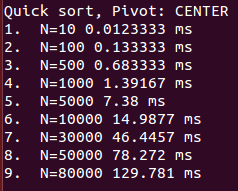
\includegraphics[width=0.35\textwidth]{center.png}
\caption{Wyniki działania programu, gdy piwot jest elementem środkowym}
\label{fig1}
\end{figure}

\item 5. Mediana z trzech. \newline
Metoda ta polega na wyliczeniu mediany z elementu najmniejszego, największego i środkowego i jego wyborze, jako elementu osiowego. Idealną sytuacją byłoby za każdym razem obliczanie mediany z całej listy, jednak takie podejście wymaga w praktyce wstępnie posortowanej tablicy do wyznaczenia mediany... (co oczywiście jest sprzeczne z celowością sortowania). Kompromisem dającym dobre rezultaty jest właśnie wyznaczenie mediany z trzech wartości. Według moich pomiarów jest to metoda najszybsza.
\begin{figure}[ht]
\centering
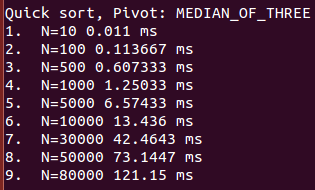
\includegraphics[width=0.35\textwidth]{median.png}
\caption{Wyniki działania programu, gdy piwot jest medianą z trzech elementów}
\label{fig1}
\end{figure}

\end{itemize}
\newpage
Dla lepszego zoobrazowania otrzymanych wyników umieszczam jeszcze wykres ze wszystkimi metodami.
\newline
\begin{figure}[ht]
\centering
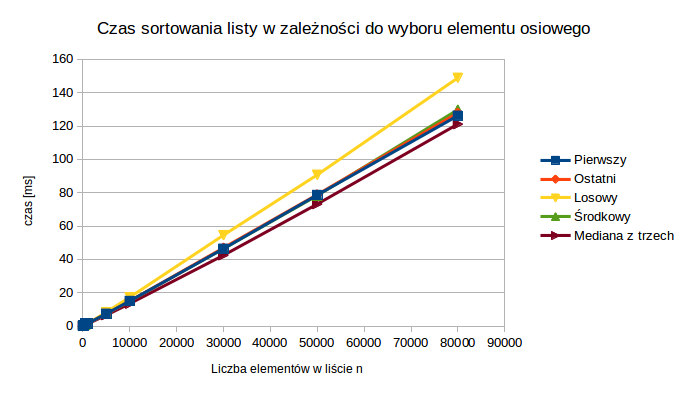
\includegraphics[width=1\textwidth]{wykres.png}
\caption{Wykres przestawiający czasy sortowania, przy różnym wyborze piwota}
\label{fig1}
\end{figure}
Możemy zaobserwować, że wszystkie metody dają dość podobne rezultaty. Dla liczb losowych najlepsza jednak (według mojej implementacji) wydaję się być metoda mediany z trzech elementów.
\end{document}